	% ---------------- Modelo Trabalho Acadêmico  - Insper ------------------ %

	% ------- Criação do documento com a classe abntex2 -------- %
	\documentclass[a4paper, 12pt, openany, oneside, brazil]{abntex2}


	% Pacotes utilizados no modelo (nem todos precisam estar presentes para a execução da sua monografia)
	\usepackage{times}			% Usa a fonte Times Roman, com compatibilidade matemática
	\usepackage[T1]{fontenc}		% Seleção de códigos de fonte.
	\usepackage[utf8]{inputenc}		% Codificação do documento (conversão automática dos acentos)
	\usepackage{indentfirst}		% Indenta o primeiro parágrafo de cada seção.
	\usepackage{color}		        % Controle das cores
	\usepackage{graphicx}			% Inclusão de gráficos/figuras.
	\usepackage{subcaption}			% Inclusão de subfiguras.
	\usepackage{microtype} 			% para melhorias de justificação
	\usepackage{amsmath}			% Pacote matemático
	\usepackage{amssymb}            % Pacote de símbolos matemáticos
	\usepackage[brazil]{babel}      % Pacote para compatibilização com a língua portuguesa
	\usepackage{setspace}           % Pacote para espaçamento entre linhas
	\usepackage{epstopdf}           % Pacote para conversão em PDF
	\usepackage{hyperref}           % Pacote para hyperlinks no documento
	\usepackage{amsthm}             % Pacote que define certos ambientes de acordo com a AMS
	\usepackage{lipsum}             % Pacote para geração de texto em grego sem sentido (só para preencher as seções)
	\usepackage{colortbl}           % Pacote que permite colorir palavras
	\usepackage{xcolor}             % Pacote para cores
	\usepackage{textcomp, gensymb}	        % Pacote para símbolos simples
	\usepackage{cancel}             % Pacote para mais notação matemática
	\usepackage[normalem]{ulem}     % Pacote para underline
	\usepackage{booktabs}           % Pacote para tabelas
	\usepackage{siunitx}            % Pacote para formatação de unidades de medida
	\usepackage{amsfonts}           % Pacote para fontes e símbolos matemáticos
	\usepackage{lastpage}           % Pacote para tomar a referência da última página
	\usepackage[font=footnotesize,labelfont=bf]{caption}
	% Pacotes de citações %
	\usepackage[brazilian,hyperpageref]{backref}	 % Paginas com as citações na bibl
	\usepackage[alf, abnt-emphasize=bf]{abntex2cite}    % Citações padrão ABNT
	\usepackage{quoting}                                % Pacote para citações

	\graphicspath{ {./images/} }

	% --------------- Definições e notações matemáticas usadas no texto -----------------%

	% Conjuntos de números naturais, racionais e reais
	\def\N{\mathbb{N}}
	\def\Q{\mathbb{Q}}
	\def\R{\mathbb{R}}

	% Símbolos letras maiúsculas caligráficas
	\def\A{\mathcal{A}}
	\def\B{\mathcal{B}}
	\def\C{\mathcal{C}}
	\def\D{\mathcal{D}}
	\def\E{\mathcal{E}}
	\def\F{\mathcal{F}}
	\def\H{\mathcal{H}}
	\def\I{\mathcal{I}}
	\def\L{\mathcal{L}}
	\def\P{\mathcal{P}}
	\def\R{\mathbb{R}}
	\def\S{\mathcal{S}}
	\def\T{\mathbb{T}}
	\def\X{\mathcal{X}}
	\def\Y{\mathcal{X}}
	\def\W{\mathcal{Z}}

	% Símbolos específicos
	\def\pf{\succcurlyeq}
	\def\ps{\succ}
	\def\ind{\sim}
	\def\inc{\not \gtrless}
	\def\pft{\preccurlyeq}
	\def\pst{\prec}
	\newcommand{\incomparavel}{\succ\kern-0.45cm \prec}

	%%% Símbolos lógicos
	\def\oulog{\vee}
	\def\elog{\wedge}
	\def\implica{\Rightarrow}
	\def\eeq{\Leftrightarrow}

	% Ambientes - Teoremas, etc. - A numeração de cada ambiente no texto é feita de acordo com o ambiente escolhido.
	\newtheorem{axiomas1}{Axioma}
	\newtheorem{teo1}{Teorema}
	\newtheorem{lema1}{Lema}
	\newtheorem{defi1}{Definição}
	\newtheorem{ex1}{Exemplo}
	\newtheorem{prop1}{Proposição}



	% ------------------ Configuração e customização dos pacotes ---------------------- %

	% Configurações do pacote backref
	% Usado sem a opção hyperpageref de backref
	\renewcommand{\backrefpagesname}{}
	% Texto padrão antes do número das páginas
	\renewcommand{\backref}{}
	% Define os textos da citação
	\renewcommand*{\backrefalt}[4]{}%


	% Customização da capa
	\renewcommand{\imprimircapa}{%
	    \begin{capa}%
	    \center{\ABNTEXchapterfont\large\imprimirinstituicao}
	    
	    \vspace*{\fill}
	    
	    \center{\ABNTEXchapterfont\large\imprimirautor}
	    
	    \vspace*{\fill}
	    {\ABNTEXchapterfont\bfseries\LARGE\imprimirtitulo}
	    \vspace*{\fill}
	    
	    {\large\imprimirlocal}
	    \par
	    {\large\imprimirdata}
	\vspace*{1cm}
	\end{capa}
	}


	% Customização do cabeçalho
	\makepagestyle{tccinsper}
	  %cabeçalhos
	  \makeevenhead{tccinsper} %%pagina par
	     {}
	     {}
	     {\thepage}
	       \makeoddhead{tccinsper} %%pagina com oneside
	     {}
	     {}
	     {\thepage}

	% Customização dos hiperlinks
	\definecolor{Lgray}{RGB}{207,207,207}
	\definecolor{black}{RGB}{0,0,0}
	\makeatletter
	\hypersetup{
			% pagebackref=true,
			pdftitle={\@title},
			pdfauthor={\@author},
			pdfsubject={\imprimirpreambulo},
			pdfcreator={LaTeX with abnTeX2},
			% pdfkeywords={abnt}{latex}{abntex}{abntex2}{relatório técnico},
			colorlinks=true,       		% false: boxed links; true: colored links
			% colorlinks=false,
			linkcolor=black,          	% color of internal links
			citecolor=black,        		% color of links to bibliography
			filecolor=magenta,      		% color of file links
			urlcolor=black,
			bookmarksdepth=4
	}
	\makeatother


	% Configuração dos espaçamentos entre linhas e parágrafos

	% O tamanho do parágrafo é dado por:
	\setlength{\parindent}{1.3cm}

	% Controle do espaçamento entre um parágrafo e outro:
	\setlength{\parskip}{0.2cm}  % tente também \onelineskip

	% Compila o indice
	\makeindex


	% Mais alguns comandos personalizados
	\newcommand*\rfrac[2]{{}^{#1}\!/_{#2}}
	\renewcommand{\arraystretch}{1.3} 			% Espaçamento na tabela
	\newcommand{\volume}{\mathop{\ooalign{\hfil$V$\hfil\cr\kern0.08em--\hfil\cr}}\nolimits} % Símbolo V cortado
	\newcommand\rlArrow[1]{$\color{red}{abc \rightarrow} #1 \color{blue}{\leftarrow} abc$}


	% Informações de dados para CAPA
	\autor{Augusto Aceituno Carneiro}
	\titulo{Título: subtítulo}
	\instituicao{
	  %
	  Insper Instituto de Ensino e Pesquisa

	  Ciências Econômicas
	  }
	\local{São Paulo - SP}
	\data{2024}

	% Informações de dados para FOLHA DE ROSTO

	\autor{Augusto Aceituno Carneiro}
	\titulo{Impacto do Impulso Fiscal na Argentina}
	\orientador{Eduardo Correia de Souza}
	\local{São Paulo - SP}
	\data{2024}

	\preambulo{Trabalho de conclusão de curso apresentado ao programa de graduação em Economia como requisito parcial para obtenção do título de bacharel em Ciências Econômicas.}


	% ------------------------------------------------------------------------------ %
	% --------------------------- Início do documento ------------------------------ %
	% ------------------------------------------------------------------------------ %
	\begin{document}

	% Retira espaço extra obsoleto entre as frases.
	\frenchspacing

	% ------------------------------------------------------------------------ %
	%                          ELEMENTOS PRÉ-TEXTUAIS
	% ------------------------------------------------------------------------ %
	\pretextual


	% Capa e Folha de Rosto
	\imprimircapa
	\imprimirfolhaderosto

	% Configuração da ficha catalográfica
	\begin{fichacatalografica}
	    \vspace*{15cm} % Posição vertical
	    \hrule % Linha horizontal
	    \begin{center} % Minipage Centralizado
	    \begin{minipage}[c]{12cm} % Largura
	    
	    \imprimirautor
	    
	    \hspace{0.5cm} \imprimirtitulo / \imprimirautor. -
	    \imprimirlocal: \imprimirdata

	    \hspace{0.5cm} \pageref{LastPage} p.

	\hspace{0.5cm}
	\parbox[t]{\textwidth}{\imprimirtipotrabalho: \ \imprimirinstituicao, \imprimirdata.}\\

	\hspace{0.5cm} \imprimirorientadorRotulo \ \imprimirorientador

	    \hspace{0.5cm}
	1. Impulso Fiscal;
	2. Argentina;
	I. Autor.
	II. Título.
	    \end{minipage}
	    \end{center}
	    \hrule
	\end{fichacatalografica}

	% Configuração da folha de aprovação
	\begin{folhadeaprovacao}

	  \begin{center}
	    {\ABNTEXchapterfont\large\imprimirautor}

	    \vspace*{\fill}\vspace*{\fill}
	    \begin{center}
	      \ABNTEXchapterfont\bfseries\Large\imprimirtitulo
	    \end{center}
	    \vspace*{\fill}
	    
	    \hspace{.45\textwidth}
	    \begin{minipage}{.5\textwidth}
		\imprimirpreambulo
	    \end{minipage}%
	    \vspace*{\fill}
	   \end{center}
		
	    \vspace*{\fill}
		
	    \begin{center}
	      \ABNTEXchapterfont\bfseries\large{Banca examinadora}
	    \end{center}
		
	    \vspace*{\fill}
	   %Trabalho aprovado. \imprimirlocal, x de x de x:

	   \assinatura{\textbf{\imprimirorientador} \\ Orientador(a)} 
	   \assinatura{\textbf{Professor} \\ Examinador(a)}
	   %\assinatura{\textbf{Professor} \\ Examinador(a)}
	   %\assinatura{\textbf{Professor} \\ Examinador(a)}
	   %\assinatura{\textbf{Professor} \\ Examinador(a)}
	      
	   \begin{center}
	    \vspace*{0.5cm}
	    {\large\imprimirlocal}
	    \par
	    {\large\imprimirdata}
	    \vspace*{1cm}
	  \end{center}
	  
	\end{folhadeaprovacao}

	\begin{agradecimentos}
	\end{agradecimentos}


	% Resumo e abstract
	% Resumo em português
	\setlength{\absparsep}{18pt} % ajusta o espaçamento dos parágrafos do resumo
	\begin{resumo}
	Políticas fiscais são instrumentos utilizados pelas autoridades políticas para alterar a dinâmica da economia e tentar controlar a dívida pública por meio de decisões sobre arrecadação de impostos e gastos públicos. Porém, a utilização desse instrumento de maneira errada pode gerar um efeito reverso e resultar em uma degradação retroalimentada da economia do país. Veremos nesse trabalho de conclusão de curso os fatores determinantes para o sucesso de uma política fiscal, explorando os efeitos da composição e do tamanho dessas políticas em seu sucesso. Em seguida, introduziremos o contexto econômico histórico da Argentina e investigaremos a maneira pela qual foram dirigidas as medidas fiscais que levaram à sua decadência econômica, comparando-as com as medidas propostas pelo recém-eleito presidente, Javier Milei, e debateremos possíveis trajetórias para a economia argentina. 

	Palavras-chave: Política Fiscal, Argentina, Javier Milei.
	\end{resumo}

	% Resumo em inglês
	\begin{resumo}[Abstract]
	 \begin{otherlanguage*}{english}
	Fiscal policies are tools used by political authorities to alter the dynamics of the economy and attempt to control public debt through decisions on tax collection and public spending. However, the misuse of this instrument can have a reverse effect and result in a self-reinforcing degradation of the country's economy. In this work, we will examine the determining factors for the success of a fiscal policy, exploring the effects of the composition and size of these policies on their success. Subsequently, we will introduce the historical economic context of Argentina and investigate how the fiscal measures that led to its economic decline were directed, comparing them with the measures proposed by the newly elected president, Javier Milei, and discuss possible trajectories for the Argentine economy.


Keywords: Fiscal Policy, Argentina, Javier Milei.
 \end{otherlanguage*}
\end{resumo}


% Insere o sumário automático
\pdfbookmark[0]{\contentsname}{toc}
\tableofcontents*
\cleardoublepage


% ----------------------------------------------------------------------- %
%                            ELEMENTOS TEXTUAIS
% ----------------------------------------------------------------------- %

\textual
\pagestyle{tccinsper} %Define o estilo da página utilizado

% ---------------------------  Introdução ------------------------------- %
% Introdução que mostra o escopo do período analisado (a partir do final dos anos noventa)
\chapter{Introdução}

A trajetória econômica da Argentina a partir do final dos anos 90 até os anos atuais é marcada por significativos desafios econômicos e uma dívida externa insustentável e crescente que levou o país a realizar o segundo maior default da história em 2001 \cite{Damill2006}. O problema da dívida pública voltou a se agravar durante o mandato de Mauricio Macri, de 2016 a 2019, e atingiu récordes de alta durante o mandato de Alberto Fernandez, de 2020 a 2023.

% Responder a pergunta: 
%     como resumir a "forma a qual políticas fiscais deterioraram a economia que não seja irresponssabilidade fiscal" 
A decadência da economia argentina não é reflexo apenas da irresponsabilidade fiscal dos governos eleitos, essa decadência se dá principalmente pela forma pela qual medidas fiscais foram adotadas pelo governo, mesmo que estas tenham sido adotadas visando a melhora da situação econômica. Quando explorarmos a literatura sobre episódios fiscais, veremos que as evidências mostram que a economia mainstream subestima o efeito de diminuição de impostos enquanto superestima o efeito do aumento dos gastos públicos \cite{Alesina1998} \cite{Ribas2021} \cite{McDermott1996}.
% o que é a "economia mainstream"? ela realmente subestima?
%     isso deve ser respondido na literatura

% o que foi o peronismo? quem fez parte? quais eram os conceitos que uniam os peronistas como um grupo e de que maneira ele agia?
A recente ascensão de Javier Milei ao poder como presidente da Argentina marcou o fim de uma longa era do peronismo, trazendo consigo novas perspectivas para a política fiscal do país. A corrente econômica seguida por Milei o faz buscar a diminuição do tamanho do estado, no contexto pessoal e principalmente no contexto econômico, visão que se opõe àquela adotada historicamente como fundamento da maioria das medidas fiscais implementadas no país.

Este trabalho busca explorar o impacto de políticas de austeridade semelhantes àquelas propostas por Milei, utilizando uma métrica de análise de políticas fiscais proposta por \cite{Blanchard1990}, o impulso fiscal. Serão utilizados dados históricos para estudar o impacto do impulso no crescimento e outras importantes variáveis econômicas.

Após a introdução, o trabalho está estruturado da seguinte forma: na seção 2, é explorada a literatura sobre o tema tratado; na seção 3 serão descritos os dados analisados e utilizados para o cálculo do impulso fiscal, contendo também um foco no histórico da economia argentina; na seção 4 será descrita a metodologia da análise, detalhando o cálculo do impulso fiscal e o Modelo Vetorial Autoregressivo (VAR) proposto para estimar o impacto do impulso fiscal nas variáveis; na seção 5 os resultados serão apresentados e analisados; por fim, a seção 6 contém as conclusões do trabalho. 

% --------------------------- Desenvolvimento ------------------------ %
\chapter{Análise da Literatura}

% Tales of Fiscal Adjustment
Em seu artigo, Alberto Alesina e Silvia Ardagna (1998) se propõem a analisar empiricamente os efeitos de mudanças discricionárias em políticas de ajuste fiscal sobre a economia utilizando o balanço primário ciclicamente ajustado pelo método de Blanchard \cite{Alesina1998}. Alesina e Ardagna identificam características dessas políticas, como: sua composição, tamanho e sucesso, descrito pelos autores como "Um período de política fiscal contracionista tem sucesso se a) nos três anos seguintes ao período, a razão entre o déficit primário ciclicamente ajustado e o Produto Interno Bruto (PIB) é, em média, pelo menos dois por cento do PIB menor do que seu valor no período da política, ou b) três anos após o período, a razão dívida/PIB está cinco por cento do PIB menor do que seu valor no período da política" \cite{Alesina1998}. As evidências encontradas pelos autores mostram que a composição do ajuste fiscal tem impacto em sua chance de sucesso muito mais expressivo do que seu tamanho, expondo que ajustes realizados com foco na redução de gastos tendem a ter chances de sucesso notadamente maiores, em especial se forem realizados através da diminuição de salários e programas de transferência públicos. Em contraste, ajustes feitos através do aumento de impostos têm chance de sucesso inferior, ou seja, não tendem a levar a uma consolidação permanente das finanças governamentais.


Como citado inicialmente na introdução deste trabalho, esses resultados encontrados pelos autores vão de encontro ao comportamento descrito pela teoria keynesiana tradicional \cite{Alesina1998}, pela qual aumentos de gastos governamentais seriam capazes de aumentar a demanda agregada, e cortes desses gastos levariam a uma contração, além de implicar que cortes em impostos deveriam ser menos expansionários que aumentos nos gastos, noção refutada pelas evidências.

% Impacto Do Impulso Fiscal Sobre O Crescimento Econômico Em Economias Emergentes E Desenvolvidas
Costa (2021) estrutura seu trabalho “Impacto do impulso fiscal sobre o crescimento econômico em economias emergentes e desenvolvidas” de forma semelhante a Alesina e Ardagna, propondo o estudo do impacto do impulso fiscal no crescimento de médio prazo (período de 5 anos proposto pelo autor) de economias emergentes e desenvolvidas também através do método de ajuste de Blanchard, analisando a possível diferença do impacto nos diferentes contextos de ajuste e expansão, assim como o mecanismo pelo qual esses foram realizados, receita ou despesa. 

Após uma análise para o período de 2000 a 2019, Costa identifica que o impulso fiscal proposto só teve impacto significativo quando separado por tipo de episódio ou considerando a atuação da política monetária no ano do episódio: em países desenvolvidos em episódios de ajustes por meio da receita ou expansões por meio da despesa, e ainda em países desenvolvidos onde o episódio fiscal expansionista foi acompanhado de uma política monetária restritiva. Os resultados significativos encontrados descrevem que, em países desenvolvidos, um aumento da receita em episódio de ajuste contribui negativamente para o crescimento no médio prazo, assim como um aumento da despesa em episódio de expansão. O resultado foi análogo ao considerar a atuação da política monetária, revelando que um aumento da despesa em um episódio de expansão, concomitante com política monetária restritiva, tem efeito negativo sobre o crescimento econômico. Adicionalmente, ainda em países desenvolvidos, Costa encontra que aumentos na folha de pagamento do governo também têm impacto negativo no crescimento econômico, ao contrário da proteção dos gastos sociais, que contribuem positivamente para o crescimento. Os achados de Costa corroboram os resultados encontrados por Alesina e Ardagna. Porém, Costa não achou significância estatística no impacto para países em desenvolvimento.

% The Argentinean Debt: History, Default and Restructuring
Damill et al. (2006), em sua análise do histórico da dívida pública argentina, colocam que as variações da trajetória econômica seguida pelos países da América Latina no pós-crise dos anos 80 foram causadas pelas políticas fiscais adotadas por cada país \cite{Damill2006}. As características do gerenciamento histórico das políticas fiscais argentinas encontradas pelos autores também corroboram os resultados encontrados por Alesina e Ardagna. Por exemplo, uma política sobre gastos com transferências públicas: a reforma de 1994 que introduziu um sistema de capitalização individual administrado por fundos de pensão privados, nomeados de "Administradoras de Fondos de Jubilaciones y Pensiones" (ADJPs) que gerou um redirecionamento das contribuições, do sistema público para o privado, que financiavam diretamente as pensões, degradando a receita do sistema de seguridade social sem alterar seu gasto. Outro exemplo é o das medidas de ajuste fiscal realizadas pelo governo eleito em 1999 aplicadas em 2000 e 2001 que, apesar de incluir cortes de gasto, também adotavam aumentos nos impostos \cite{Damill2006}. 

% An Empirical Analysis Of Fiscal Adjustment
Expandindo também na análise empírica dos ajustes fiscais, McDermott e Wescott (1996) se deparam com as mesmas dinâmicas encontradas na literatura citada \cite{McDermott1996}, principalmente com os resultados de Alesina e Ardagna, apesar de que, ao contrário destes, os resultados de McDermott e Wescott mostrarem que o tamanho do ajuste é fator relevante na determinação de sua chance de sucesso. Os autores também exploram a possível relação entre o cenário econômico mundial e a efetividade dos ajustes, encontrando que, apesar de haver certa relação entre estes, as evidências indicam que a magnitude e composição dos ajustes ainda parecem ser os fatores dominantes.

Assim como Alesina e Ardagna, McDermott e Wescott também analisam a trajetória de variáveis macroeconômicas, antes, durante e depois dos episódios fiscais, desta vez separando-os por: de ajuste, bem e mal-sucedido; e de estímulo, endividante e neutro em termos de dívida. Os autores encontraram melhora em todas as variáveis após todos os episódios de ajuste fiscal bem-sucedido, já nos casos de: episódio de ajuste mal-sucedido, estímulo endividante e estímulo neutro na dívida, as poucas melhoras encontradas foram muito inferiores, de resto não houve alteração relevante nas variáveis ou houve piora nessas, com o caso de piora sendo o mais representativo dos resultados.




% -------------------------- Dados --------------------------- %
\chapter{Dados fiscais}

% Explicação de onde cada dado veio, se foi obtido, de onde, se foi calculado, como.
\section{Fontes e cálculos}

Os dados do PIB nominal foram obtidos pelo \textit{Portal de Datos Económicos} do ministério da economia da Argentina. Para obter uma série temporal trimestral contínua do período de 1993 até 2024 foram utilizadas duas séries de PIB a preços correntes em milhões de pesos. A primeira série se estende de 1993 até 2012, a segunda é referente a uma mudança de metologia ocorrida em 2004, e se estende de 2004 até o segundo trimestre de 2024. Foram considerados os valores da primeira série de 1993 até 2004, e a conciliação das séries foi feita ajustando a primeira, utilizando uma razão calculada entre as séries no primeiro trimestre de 2004

Os valores para receitas e gastos públicos foram elaborados pela Secretaria da Fazenda argentina e obtidos também pelo \textit{Portal de Datos Económicos}, com periodicidade trimestral de 1993 até o segundo trimestre de 2024. Houveram duas mudanças na metodologia de cálculo no período, nos anos de 2007 e 2017, não foram realizados ajustes para conciliação das séries. Os dados utilizados são de receitas e gastos primários após figuratórios, isto é, são subtraídos de valores financeiros referentes a juros e amortizações, contando apenas com valores operacionais do Setor Público Nacional argentino, ideal para análise do efeito da condução fiscal. Os valores para as séries estão a preços correntes em milhões de pesos.

O Índice de Preços ao Consumidor (IPC) também foi obtido pelo \textit{Portal de Datos Económicos}, porém não foi utilizado o IPC a nível nacional calculado pela entidade pública central de dados estatísticos da Argentina, o \textit{Instituto Nacional de Estadística y Censos de la República} (INDEC), pois há grande desconfiança nos valores disponibilizados no período de 2007 a 2015, devido à perda de autonomia e neutralidade do INDEC nos métodos de pesquisa e cálculo do IPC, resultante de intervenções do governo impostas pelo então presidente Néstor Kirchner \cite{Daniel2019}. Desta forma, foram considerados três índices de preços medidos por agências alternativas para atuar como proxy do IPC nacional: o da Província de Túcuman, o de Gran Resistencia, e o da Província de Jujuy. Após analisar a correlação de cada um com o IPC calculado com a nova metologia do INDEC iniciada em dezembro de 2016, foi escolhido o índice elaborado pela Província de Túcuman.

A dívida bruta e a dívida externa foram obtidas também pelo \textit{Portal de Datos Económicos}.

A inflação foi calculada através da variação em percentual do IPC. O IPC também foi utiizado para calcular o deflator, afim de remover os efeitos da inflação das séries do PIB, dos gastos e das receitas públicas, fixandos valores em pesos argentinos (ARS) do segundo trimestre de 2024, assim obtendo os valores reais das séries.

Devido à periodicidade trimestral das séries do PIB, receitas e gastos, faz-se necessário remover os efeitos introduzidos pela sazonalidade natural da economia, para tal, foi utilizado o método \textit{X13-ARIMA-SEATS}, através da biblioteca \textit{statsmodels} em python.

O hiato do PIB, variável utilizada pra mensurar oscilações cíclicas da economia, foi calculado com uma estimação do PIB potencial $Y^*_t$ obtida através da aplicação do filtro Hodrick-Prescott (HP) na série histórica do PIB real $Y_t$ obtendo sua tendência de longo prazo. Para este trabalho foi utilizado o filtro HP, também da biblioteca \textit{statsmodels}, com parâmetro de suavização $\lambda = 1600$ para dados trimestrais. Com o PIB potencial obtido, calculamos o hiato através da seguinte equação:

\begin{equation}
	\text{Hiato}_t = \frac{Y_t - Y^*_t}{Y^*_t}
\end{equation}

Em seguida, para que as séries de receitas e gastos públicos representem mais fielmente a condução das políticas fiscais, é necessário remover o ruído informacional introduzido por oscilações cíclicas da economia. Para isso, será utilizado o método de ajuste pela elasticidade ao hiato do PIB, proposto pelo FMI \cite{fedelino2009computing} e Blanchard e Perotti \cite{Blanchard2002}, \cite{Blanchard1990}. Esse método consiste em utilizar o hiato do PIB como mensurador dos ciclos econômicos, e coeficientes de elasticidade dos gastos e receitas públicos a esses ciclos. Assim, para o cálculo das receitas e despesas ajustadas $T^\text{adj}_t$ e $G^\text{adj}_t$, respectivamente, foram utilizados o hiato calculado, a estimativa para o coeficiente de elasticidade ao hiato das receita $\rho_T=1.23$ fornecidos pela CEPAL \cite{Martner2004}, e o coeficiente de elasticidade dos gastos $\rho_G=1.03$ calculado usando a estimativa da elasticidade do balanço primário, também da CEPAL. O cálculo do ajuste se dá pelas fórmulas:

\begin{equation}
	T^\text{adj}_t = T_t - \rho_T \cdot T_t \cdot \text{Hiato}_t
\end{equation}

\begin{equation}
	G^\text{adj}_t = G_t - \rho_G \cdot G_t \cdot \text{Hiato}_t
\end{equation}

A escolha de usar as variáveis no mesmo período fundamenta-se na premissa de que as alterações no hiato contribuem para variações nas receita e despesa no mesmo período. Ainda, foi escolhido não calcular o saldo primário, mantendo as variáveis do saldo separadas, a fim de analisar separadamente o impacto de cada posicionamento fiscal, focando nas evidências encontradas na literatura que descrevem que a escolha do instrumento a ser alterado pela política fiscal, receitas ou gastos, tem impacto mais significativo do que seu tamanho.

Após a obtenção das séries em valores reais dessazonalizados ciclicamente ajustados, foram utilizados dados históricos da população da Argentina disponibilizados pelo \textit{Our World in Data} para transformar as séries de PIB, gastos e receitas em valores per capita, para remover efeitos nas variáveis causados pela variação da população.

\section{Histórico da Condução Fiscal na Argentina}
% aqui é maneiro colocar políticas do tipo "deram subsídio pra energia ficar mais barata" e mostrar que os preços de energia subiram

A trajetória econômica argentina, da metade dos anos 90 até a recente eleição do presidente Javier Milei, foi marcada por diferentes conduções fiscais. O período do ano de 1994 até 1999 foi governado por Carlos Menem, que assumiu a presidência após a crise de 1980, em 1989. O início de seu governo foi marcado por se diferenciar do populismo anterior, através do controle dos gastos públicos e privatizações de empresas estatais, essas medidas trouxeram controle da inflação e das contas públicas no curto prazo. Menem também instaurou o Plano de Convertibilidade, que instituia a paridade fixa do peso argentino para o dólar americano e teve grande força para segurar a hiperinflação que o país vinha sofrendo. Porém, ao final de seu mandato, Menem realizou um aumento de gastos com programas sociais para manter apoio popular, o que resultou numa deteriorização das contas públicas. No gráfico a seguir, com os valores ajustados ciclicamente para as receita e gastos públicos, é possível acompanhar a trajetória do balanço primário do governo argentino no mandato de cada presidente do país.

\begin{figure}[h!]
	\caption*{Gráfico 1: Valores do balanço fiscal ajustado (em milhões de ARS)}
	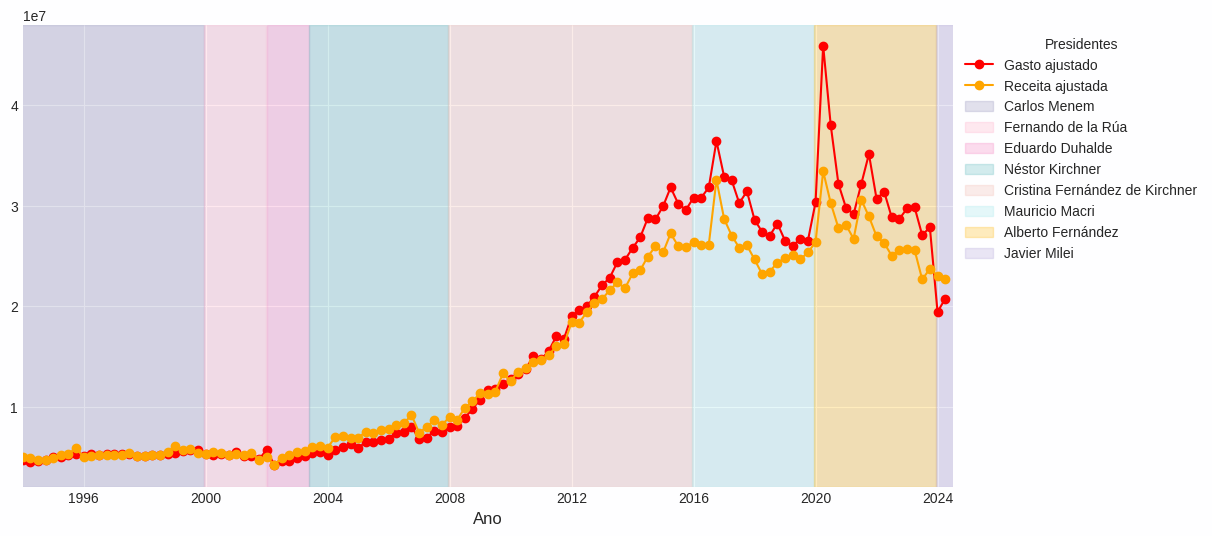
\includegraphics[width=\textwidth]{dados/valores_fiscais_ca}
	\caption*{Fonte: elaborado pelo autor}
\end{figure}

A insistência de Menem no Plano de Convertibilidade o fez recorrer ao envididamento externo (Gráfico 2) para manter a paridade da moeda, mais de 23 bilhões de dólares foram aportados no período de 1994 até 2001, com mais de 40\% desse valor concentrado no ano de 2001 \cite{Damill2006}. O financiamento do déficit com dívida externa levou o país a uma crise financeira e colapso econômico no início dos anos 2000. Seu sucessor, Fernando de la Rúa, herdou este alto endividamento, e aplicou algumas medidas de austeridade na tentativa de controlar as contas públicas, visível na redução brusca dos gastos no gráfico 1, através da redução de salários para o funcionalismo público e também de gastos com programas sociais. Porém, De la Rúa continuou o financiamento do déficit público com dívida externa iniciado no governo anterior. Fernando também aumentou impostos, refletindo em um leve aumento da receita (Gráfico 1), apesar da diminuição da atividade devido à crise (Gráfico 3).

\begin{figure}[h!]
	\caption*{Gráfico 2: Dívida externa (em milhões de ARS)}
	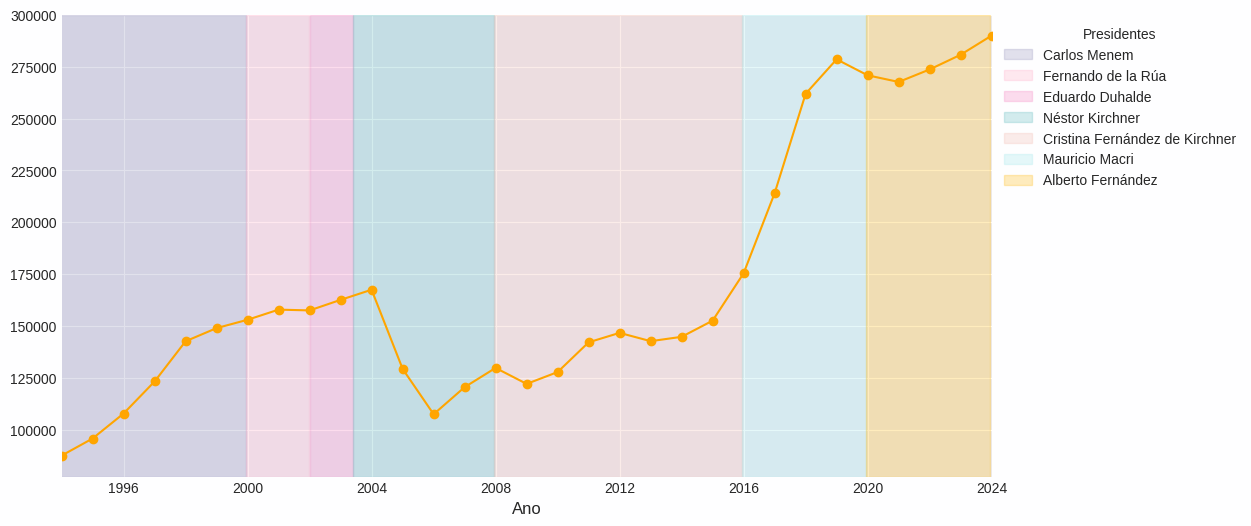
\includegraphics[width=\textwidth]{dados/divida_externa}
	\caption*{Fonte: FMI, elaborado pelo autor}
\end{figure}

\begin{figure}[h!]
	\caption*{Gráfico 3: PIB Real (em milhões de ARS)}
	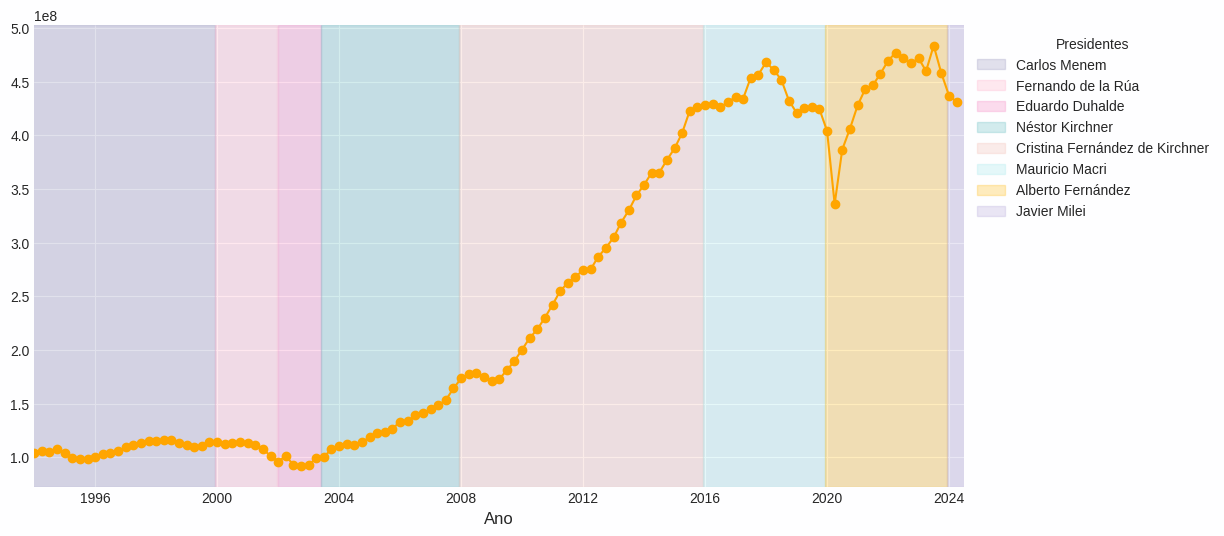
\includegraphics[width=\textwidth]{dados/pib_real}
	\caption*{Fonte: Banco Mundial, elaborado pelo autor}
\end{figure}

Após a renúncia de De la Rúa, do dia 21 de dezembro de 2001 até o dia 2 de janeiro de 2002, a Argentina teve uma série de três presidentes. Adolfo Rodríguez Saá foi o presidente escolhido pelo congresso após a renúncia de De la Rúa, e governou de 23 até 31 de dezembro de 2001. Em seu mandato, Rodriguez declarou a moratória da dívida externa, marcando o maior default soberano da história até o momento, totalizando cerca de 100 bilhões de dólares \cite{IMFArgentina2004}, atualmente estando ainda em segundo lugar.

Eduardo Duhalde assume a presidência em 2002 e encerra a paridade cambial, permitindo a flutuação do peso argentino e gerando uma forte desvalorização monetária, refletindo em um efeito inflacionário imediato (Gráfico 4).

\begin{figure}[h!]
	\caption*{Gráfico 4: Inflação (Variação trimestral do índice em \%)}
	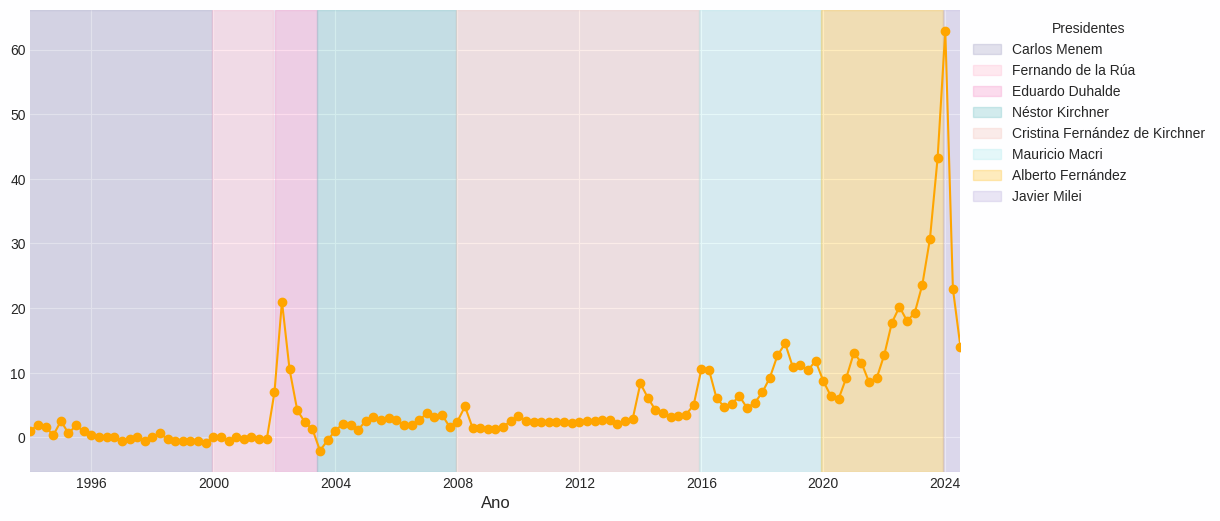
\includegraphics[width=\textwidth]{dados/inflacao}
	\caption*{Fonte: Banco Mundial, elaborado pelo autor}
\end{figure}

A rápida desvalorização do peso argentino, causada pela correção dos preços na ausência da paridade cambial, fez subir o valor em pesos argentinos de parte da dívida pública que era denominado em dólares (Gráfico 5)

\begin{figure}[h!]
	\caption*{Gráfico 5: Dívida pública (\% do PIB)}
	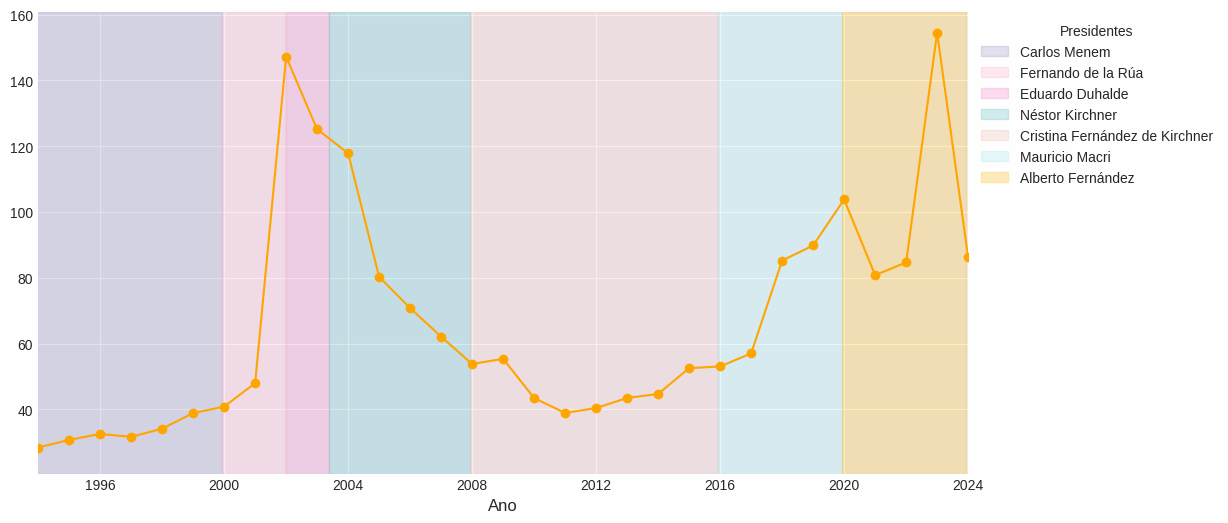
\includegraphics[width=\textwidth]{dados/divida_publica}
	\caption*{Fonte: FMI, elaborado pelo autor}
\end{figure}

O legado de Eduardo Duhalde para seu sucessor, Néstor Kirchner, foi uma profunda crise econômica. Embora ligeiramente mais controlada por seus esforços de ajustes fiscais, negociações com o FMI e tentativas de fortalecer a independência do Banco Central, a inflação permanecia alta e persistente, resultado do colapso de 2001 e do calote argentino ao FMI.

O governo de Néstor Kirchner foi marcado por elevados gastos públicos. Seguindo uma abordagem heterodoxa, o objetivo principal era o aumento da atividade econômica, negligenciando o persistente déficit primário e financiando os gastos do governo com expansão monetária. Além disso, para o controle da inflação, foram utilizados controles de preços em setores-chave e nacionalizações de empresas estratégicas, como a Aerolíneas Argentinas. Também, houve o fortalecimento das indústrias nacionais com o objetivo de promover a substituição de importações. Essas medidas explicam a alta inflação no período, o crescimento do PIB e a generosa redução da dívida pública.


Cristina Kirchner, sua sucessora, seguiu com medidas de forte intervenção estatal, expandindo ainda mais os gastos públicos e subsídios. Isso, em grande medida, foi mascarado pelo expressivo crescimento do PIB e pela expansão monetária, que contribuíram para uma inflação persistente, porém constante, durante seu primeiro mandato, até se descontrolar no ponto de inflexão de 2013. No gráfico, é evidente o aumento exponencial dos gastos do governo de 2007 a 2015, durante seus dois mandatos consecutivos. Observa-se que o controle de preços, a desconsideração do resultado fiscal e a política monetária frouxa comprometeram a estabilidade econômica de longo prazo. Essas hipóteses serão testadas sob a ótica fiscal mais adiante.


Com toda a desordem e incerteza permeando a conjuntura macroeconômica, Mauricio Macri foi eleito com a missão de executar reformas estruturais, promover a abertura econômica e alinhar a Argentina com o mercado internacional. O governo Macri foi marcado por uma política fiscal apertada: redução de gastos do governo e aumentos de impostos, incluindo a eliminação de subsídios, reforço da independência do Banco Central (adotando um regime de metas de inflação) e desvalorização do peso argentino. No gráfico, nota-se claramente o ajuste fiscal com a expressiva redução dos gastos e aumento das receitas do governo.

No entanto, mesmo com esses ajustes, Macri não conseguiu conter a inflação no curto prazo nem o crescimento da dívida pública argentina. A explicação para isso reside no fato de que, como é comum em ajustes fiscais de curto prazo, o remédio costuma ser amargo no começo: a desvalorização do peso pressionou o aumento do preço dos importados, a redução do controle de preços levou ao aumento dos preços de energia e combustíveis, e o governo já não dispunha mais do instrumento da expansão monetária para suavizar os impactos.

Enfim, com o aparente fracasso de Macri em estabilizar a moeda e sair da recessão, o país, desacreditado, abraçou novamente a forte intervenção estatal e o afrouxamento fiscal no governo de Alberto Fernández, retomando também a intervenção no mercado cambial e impondo taxas de câmbio diferenciadas. Isso resultou na escalada da dívida pública da Argentina.

Atualmente, com a insatisfação geral em relação à persistente inflação e à descredibilidade internacional, Javier Milei foi eleito na Argentina com a promessa de executar profundas reformas na economia e conter a hiperinflação iniciada no final do governo Fernández. Isso traz a oportunidade de investigar o impacto do impulso fiscal nas principais variáveis macroeconômicas e elucidar o possível impacto de um aperto fiscal pelo governo Milei.


% -------------------------- Metodologia --------------------------- %
\chapter{Metodologia}
% aqui vou introduzir o VECM, citar que é uma extensão do VAR, um modelo de regressão multivariado que trata todas as variáveis como interdependentes (dá pra falar do blanchard e bancos centrais ainda), porém, além de ser capaz de capturar relações de curto prazo, o VECM incorpora relações de longo prazo entre as variáveis, e é mais indicado pra lidar com séries temporais cointegradas, em outras palavras, séries que possuem relações estáveis de longo prazo Aqui vou citar também o teste de cointegração de johansen, que confirmou presença de cointegração entre as séries de gastos e receitas

Variáveis econômicas interagem entre si através de mecanismos complexos, e muitas vezes, essas interações não são corretamente capturadas quando analisadas através de métodos mais simples, como regressões lineares. O Modelo Vetorial de Correção de Erros (VECM) é uma extensão do modelo Vetorial Auto-Regressivo (VAR), que é um modelo de regressão multivariado que trata todas as variáveis como interdependentes, e desta forma, é capaz de capturar melhor as interações das variáveis. O VAR é utilizado na literatura para estimação do efeito de choques fiscais na economia \cite{Blanchard2002}, e historicamente por bancos centrais para estimações de crescimento e comportamento da economia, assim como análises do possível resultado de políticas fiscais e monetárias \cite{bcb_relatorio_inflacao_2010}. Porém, apesar de ser adequado para relações de curto prazo, o VAR possui limitações ao analisar séries com relações de longo prazo. O VECM, por sua vez, incorpora essas relações de longo prazo no modelo, sendo capaz de lidar com séries temporais cointegradas, ou seja, séries que possuem relações estáveis de longo prazo.

Uma importante ferramenta disponibilizada pela utilização de modelos vetoriais que incorporam relações dinâmicas entre as variáveis é a Função Impulso-Resposta (IRF), que nos permite analisar o comportamento de variáveis de interesse diante de choques nas variáveis do sistema. A IRF será utilizada aqui para estimar o efeito que choques nos gastos e receitas do governo tem no PIB per capita argentino.

Para todos os teste de hipótese que se seguem, será adotado um intervalo de confiança de 95\%.

Afim de estabilizar a variância das variáveis no tempo, foi aplicada uma transformação logaritmica, resultando na seguintes séries:

\begin{figure}[h!]
	\caption*{Gráfico 6: Logaritmo das séries}
	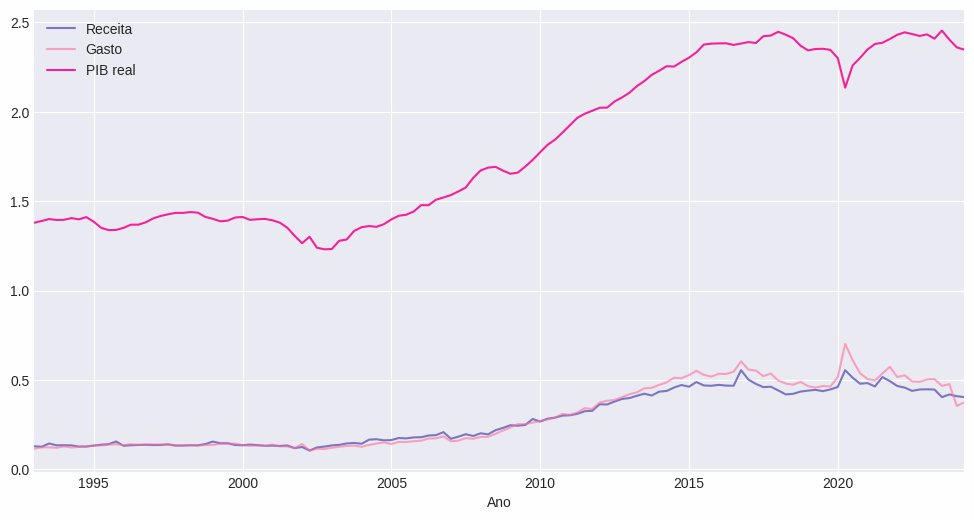
\includegraphics[width=\textwidth]{metodologia/logaritmo}
	\caption*{Fonte: Elaborado pelo autor}
\end{figure}

Como pode ser visto no gráfico, e confirmado com a aplicação de um teste Dickey-Fuller aumentado, as séries apresentam raízes unitárias, e com um teste de cointegração de Johansen, foi corroborada a presença de cointegração entre as séries das receitas e gastos. Em seguida, foram testadas ordens para o modelo até um lag máximo de 20 períodos, ou seja, cinco anos, de acordo com o tempo de resposta utilizado na literatura vista. Para selecionar a ordem mais adequada, foi utilizado o Critério de Informação de Akaike (AIC). O teste de traço foi utilizado para definir o rank de cointegração das séries. A ordem ótima encontrada foi 20, enquanto o rank de cointegração foi 2. A equação do modelo ajustado ficou: 


% \begin{equation}
% 	\text{equação do bagulho aqui}
% \end{equation}
%
%
% --------------------------- Resultados --------------------------- %
\chapter{Resultados}
Para averiguar a confiabilidade dos resultados, foi realizada uma análise dos resíduos do modelo, que nos permite ver se existe alguma relação não capturada pelo modelo e definir se os intervalos de confiança estimados para as IRF serão confiáveis. Testes de Ljung-Box confirmaram que não existe auto-correlação dos resíduos das séries, e testes de Anderson-Darling confirmaram a normalidade de suas distribuições. Assim, as IRF e seus intervalos de confiança são estatisticamente confiáveis. Desta forma, os gráficos das Funções de Impulso-Resposta e discussões sobre os resultados estão disponibilizados a seguir.


\begin{figure}[h!]
	\caption*{Gráfico 7: Resposta do PIB, Choque nas receitas públicas}
	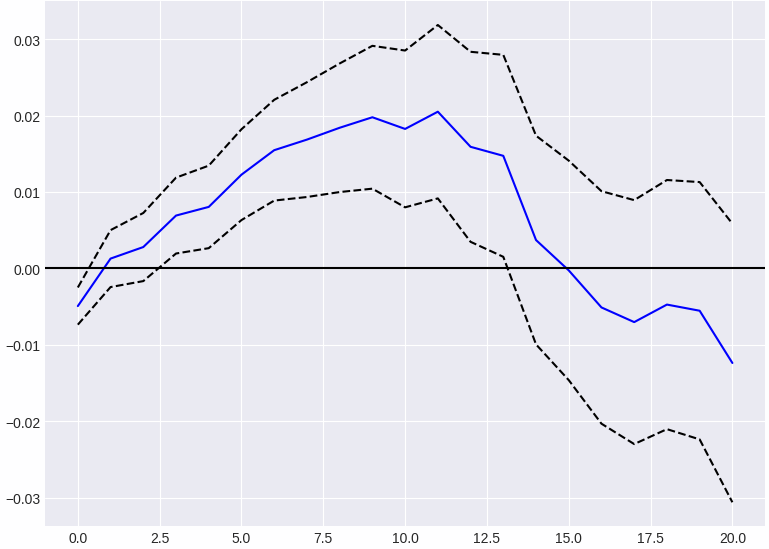
\includegraphics[width=0.75\textwidth]{resultados/irf_revenue_gdp}
	\caption*{Fonte: Elaborado pelo autor}
\end{figure}

O eixo Y representa a amplitude do efeito ao choque, enquanto o eixo X representa o intervalo de tempo após o choque. Por conseguinte, o gráfico da IRF acima descreve que um choque nas receitas públicas per capita tem efeito negativo no mesmo período no PIB real per capita, porém, gera um efeito positivo a partir do terceiro trimestre após o choque, que se mantem até o décimo terceiro trimestre (início do quarto ano), quando o efeito positivo é diluído e o PIB volta à média com aparente tendência de queda. Os impactos a longo prazo (mais de cinco anos) são inconclusivos, pois apesar de uma aparente forte tendência de queda do PIB, o intervalo de confiança engloba o valor zero, indicando possível ausência de significância estatística.

\begin{figure}[h!]
	\caption*{Gráfico 8: Resposta do PIB, Choque nos gastos públicos}
	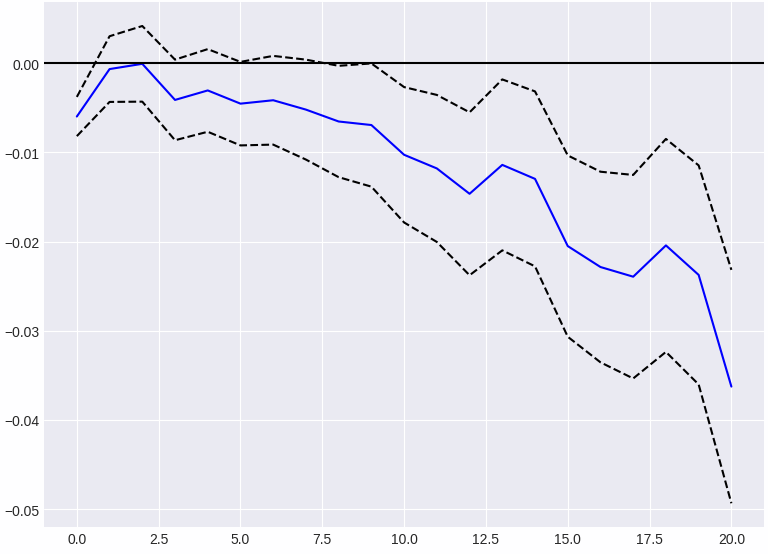
\includegraphics[width=0.75\textwidth]{resultados/irf_expenditure_gdp}
	\caption*{Fonte: Elaborado pelo autor}
\end{figure}

O gráfico da resposta do PIB a choques nos gastos públicos descreve um efeito quase exclusivamente negativo, iniciando no mesmo período do choque, e tornando a demonstrar um efeito negativo estatisticamente significativo a partir do nono trimestre (início do terceiro ano) após o choque, arrastando esse efeito negativo para o longo prazo.



% --------------------------- Conclusão ---------------------------- %
\chapter{Conclusão}
Os resultados encontrados estão de acordo com a literatura sobre o tema, corroborando que políticas fiscais de aumento de gastos e aumento de impostos geram efeitos negativos na atividade econômica de médio (gastos e impostos) e longo prazo (gastos). 

O efeito prático do aumento sistêmico da atuação do estado na economia por meio de aumento de gastos e impostos é a diminuição da participação dos agentes naturais da iniciatva privada. Como as instituições governamentais não estão sujeitas aos sinais naturais dos mercados, o que ocorre com uma economia com o crescimento da participação estatal é a diminuição da eficiência do processo natural de mercado.

É possível que as medidas tomadas por Javier Milei permitam a volta da atuação dos agentes da iniciativa privada no mercado. Independente do resultado de seu governo, suas políticas serão um interessante estudo de caso para analisar a condução de políticas fiscais

% Todos os códigos e dados usados neste trabalho estão disponíveis em https://github.com/cwrneiro/tcc


% ------------------------------------------------------------------- %
%                       ELEMENTOS PÓS-TEXTUAIS
% ------------------------------------------------------------------- %
\postextual


% Bibliografia
\bibliography{bib} % sem a extensão .bib

% Apêndices
% \begin{apendicesenv}
%
% Imprime uma página indicando o início dos apêndices
% \partapendices



% \end{apendicesenv}



% Anexos

% \begin{anexosenv}
% 
% Imprime uma página indicando o início dos anexos
% \partanexos
% 
%
% \chapter{Capítulo anexo 1}


% \end{anexosenv}

% \bibliography{bibliografia}


% \begin{apendicesenv}

% % Imprime uma página indicando o início dos apêndices
%\partapendices

\end{document}
